\documentclass[11pt]{article}

% Other packages for formatting
\usepackage[margin=1in]{geometry}
\usepackage{setspace}
% \onehalfspacing
\linespread{1.15}
\usepackage{fancyhdr}
\usepackage{graphicx}             % For including images
\usepackage{titlesec}             % For customizing section titles

\usepackage{amsmath, physics, amssymb}

% Set up the custom page style for the first page
\fancypagestyle{firstpagestyle}{
    \fancyhf{} % Clear all headers and footers
    \fancyhead[L]{\LARGE \textbf{Research Statement}}
    \fancyhead[R]{\Large \href{https://www.mathisgerdes.com}{\textbf{Mathis Gerdes}}}
    \renewcommand{\headrulewidth}{0pt} % Remove the default header rule
    \fancyfoot[C]{- {\thepage} -}
}

% Regular page style for the rest of the document
\pagestyle{fancy}
\fancyhf{} % Clear all headers and footers
\fancyhead[L]{\textbf{Research Statement}} % Regular header on subsequent pages
\fancyhead[R]{\textbf{Mathis Gerdes}}
\fancyfoot[C]{- {\thepage} -}

\usepackage{xcolor}
\definecolor{royalblue}{rgb}{0.2, 0.3, 0.7} % Adjust the RGB values for your preferred shade of blue
\usepackage[colorlinks=true, linkcolor=royalblue, urlcolor=royalblue, citecolor=royalblue]{hyperref}
\usepackage[colorlinks=true, linkcolor=royalblue, urlcolor=royalblue, citecolor=royalblue]{hyperref}

\usepackage{parskip}
\usepackage[sort&compress,numbers]{natbib}
\setlength{\bibsep}{2pt}

% Title information
\title{}
\author{}
\date{}

\begin{document}
\thispagestyle{firstpagestyle}


My research seeks to address complex questions in quantum field theory and string theory by pioneering computational and machine learning techniques, enabling new insights into non-perturbative regimes.
My experience spans lattice quantum chromodynamics (QCD) and string compactifications, where sophisticated tools are essential to push forward theoretical insights.

Advances in computational paradigms and hardware driven by machine learning are unlocking new
ways to tackle key challenges in theoretical physics. My goal is to create novel computational
frameworks that push the boundaries of quantum field theory and theoretical physics. To achieve
this, I will draw on my broad experience with emerging machine learning techniques for scientific
problems, as well as my strong background in both theoretical physics and computer science.

\paragraph{\textit{{Calabi-Yau Metrics.}}}
Calabi-Yau manifolds play a crucial role in string compactifications.
Their geometric structure encoded in the metric is not known analytically, but is required for example to determine the Yukawa couplings of the low-energy effective theory.
This led me to devise novel machine learning methods to approximate Ricci-flat metrics on these manifolds.
By expressing a spectral ansatz that inherently guarantees important differential properties as a trainable neural network, I achieved higher accuracies than established methods more efficiently by simultaneously learning their moduli dependence.
This achievement was made possible by my efficient numerical implementation of intricate mathematical structures such as sections of holomorphic line bundles on complex projective spaces, metrics in local coordinate patches and derived geometric properties like the Ricci curvature.
Building on initial work during my MSc in theoretical and mathematical physics at the LMU Munich, I have since published a library of these computational methods \cite{gerdes2023CYJAXPackage} and co-authored an influential article explaining different machine learning approaches to this problem in collaboration with international collaborators \cite{anderson2021ModulidependentCalabiYau}.

\textbf{\color{royalblue}{Future Directions.}}
A rich space of mathematical constructions of Calabi-Yau manifolds remains to be explored, including the extension of my spectral method to complete intersection Calabi-Yau manifolds.
The field of AI applications in string theory and mathematics is becoming increasingly rich.
In this context, it appears to me that the utilization of long-established ideas in metaheuristics such as particle swarm optimization, simulated annealing and evolutionary algorithms remain under-explored.
I therefor aim to investigate, in particular, how these methods may be leveraged in the context of conformal bootstrap and the search for string vacua.

\paragraph{\textit{{Lattice Quantum Field Theory and Non-Perturbative QCD.}}}
Quantum chromodynamics in the non-perturbative regime remains one of the most challenging and important areas of theoretical physics.
Lattice QCD provides a powerful framework for exploring this regime, but computational limitations have historically restricted our ability to fully explore it.
In my research, I have pioneered continuous normalizing flows for learning the complex distributions arising in lattice quantum field theory. By building the symmetries of the discretized theory directly into a trainable ordinary differential equation that parametrizes the field transformations, I have demonstrated state of the art performance on scalar theories \cite{gerdes2023LearningLattice}.

I have recently extended this work to gauge theories, developing flexible gauge-equivariant continuous flows \cite{gerdes2024continuousGauge}.
To achieve this, I implemented an integration scheme for matrix group manifolds that facilitates efficient gradient computation by leveraging modern ML libraries, and designed a new gauge-equivariant ODE architecture that delivers state-of-the-art sampling quality.
A continuous flow on a single SU(3) element is shown in Figure \ref{fig:su3}.

\begin{figure}
    \centering
    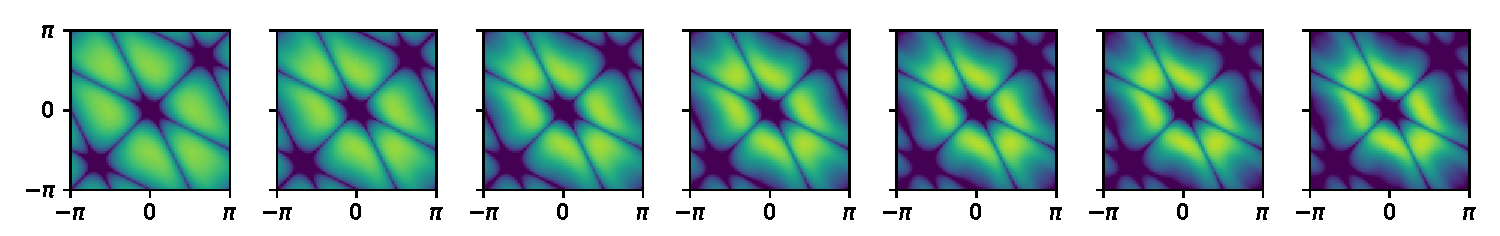
\includegraphics[width=\linewidth]{su3.pdf}
    \vspace{-25pt}
    \caption{\footnotesize Density of conjugation equivariant continuous flow on SU(3) in angular coordinates along flow time.}
    \label{fig:su3}
    \vspace{-10pt}
\end{figure}

\textbf{\color{royalblue}{Future Directions.}}
I will continue this work with my collaborators by addressing the problem of scaling up to larger lattice sizes, including exploring multi-scale generation, transfer learning, and the thermodynamic properties of these flows, as well as their deeper connection to the renormalization group (RG). Leveraging the structural overlap in mathematical concepts, I have also recently become excited about the prospect of combining my experience in the context of Calabi-Yau manifolds to improve sampling for $\mathbb{CP}^N$ models, which suffers from topological freezing.

I am excited to explore how these sampling methods developed in the context of lattice quantum field theory can be applied in condenced matter problems more broadly.
In particular, the idea of inverse RG has shown recent success for spin glass models.
This is closely related to the problem of scaling up to larger lattice sizes, which is present in both cases.

Modeling neural wavefunctions using techniques similar to generative models has shown success in fields such as quantum chemistry and many-body systems. Exploiting the technological overlap, I aim to extend our methods developed for generative models to explore neural wavefunctions for lattice QCD. This could provide a new approach to mitigate the sign problem.

\paragraph{\textit{{Interdisciplinary Research Bridging Theory and Computation.}}}
I enjoy applying my knowledge across domain boundaries.
For example, informed by my work on generative models for lattice quantum field theory, I have explored connections between RG and diffusion models.
This led me to developed a generalized RG-inspired framework for diffusion models \cite{gerdes2024gudgenerationunifieddiffusion}, in collaboration with Prof Max Welling, that enlarges the design space for diffusive processes and makes explicit its sequential nature.
Another example of interdisciplinary work I have enjoyed is in statistical data analysis and in particular simulation based inference, which incorporates machine learning to tackle large numbers of nuisance parameters that can arise from more faithful physical models.
In this context, I have developed an efficient simulator for stellar streams evolving in a gravitational background, to advance theoretical insight derived from astrophysical observations  \cite{alvey2023AlbatrossScalable}.
This led me to study theoretical statistics and differences between frequentist and Bayesian approaches in this field.
Having discovered an interesting dual point of view between these, I am presently studying optimization schemes that combine and unify notions from both frequentism and Bayesianism.

\bibliographystyle{abbrvnat-sorted}
{
    \small
    \bibliography{refs}
}

\end{document}
